% !TeX root = ../main.tex
% =====================================================================
% Chapter 5 -- Base Operating System: Axcan OS  (restructured)
%
% Preamble: same as Chapter 4 (amsmath, amssymb, booktabs, graphicx,
% hyperref, cleveref, and the assumption/requirement counters).
% =====================================================================

\chapter{Base Operating System: Axcan OS}\label{chap:os}

The architecture developed in Chapter~\ref{chap:approach} requires an
execution platform on every node. That platform must satisfy
\cref{req:portability} --- the same task binary must run on physical and
virtual nodes alike --- and provide the mechanisms on which
\cref{req:transfer,req:state,req:criticality} depend: it must be able to
receive and start a task it was not compiled with, to preserve and restore
that task's state, and to schedule tasks of differing criticality without
allowing the less critical to interfere with the more critical. It must do so
within a footprint appropriate to ECU-class hardware
(\cref{req:footprint}).

This chapter describes Axcan OS, the platform developed to meet these
requirements.\footnote{The name derives from the Nahuatl \textit{axcan},
meaning \emph{now} or \emph{immediately}.} Section~\ref{sec:os:rationale}
states its relationship to the software it builds on.
Section~\ref{sec:os:architecture} presents the architecture.
Sections~\ref{sec:os:scheduler} to~\ref{sec:os:guesttask} describe the four
mechanisms that distinguish Axcan OS from its base: the mixed-criticality
scheduler, dynamic task deployment, cross-platform task loading, and the guest
task model. Sections~\ref{sec:os:isolation} to~\ref{sec:os:footprint} address
memory management and isolation, failure handling, and resource footprint.

% =====================================================================
\section{Design Rationale and Relationship to Existing Software}
\label{sec:os:rationale}

The choice of FreeRTOS as the base kernel was argued in
Section~\ref{sec:designdecisions}; the argument is not repeated here. What
matters for this chapter is the gap between what FreeRTOS provides and what
the architecture requires.

FreeRTOS provides deterministic scheduling, task and queue primitives, and
ports to a wide range of hardware, at a footprint of a few tens of kilobytes.
It does not provide the following. Applications are compiled into the kernel
image, so a node cannot execute a task it did not ship with. Scheduling is
fixed-priority, with no priority-assignment policy and no notion of
criticality. There is no mechanism for preserving task state across anything.
And although the kernel itself is portable, the services an application needs
--- console output, networking, memory allocation --- are reached through
platform-specific interfaces, so an application compiled against one port will
not run on another.

Axcan OS closes these four gaps. Its relationship to the software it builds on
is as follows:

\begin{itemize}
  % TODO: insert the FreeRTOS version number after "FreeRTOS" below.
  \item \textbf{FreeRTOS} supplies the kernel: threading,
    context switching, queues, and the hardware ports used for both the
    embedded and the POSIX targets. It is used unmodified except
    where noted in Section~\ref{sec:os:isolation}.
    % TODO: state the FreeRTOS version and whether the kernel was patched.

  \item \textbf{ESFREE}~\parencite{esfree} supplies the scheduling framework.
    ESFREE replaces the fixed-priority scheduler of FreeRTOS with a policy
    layer supporting static and dynamic real-time policies, among them
    rate-monotonic, deadline-monotonic and Earliest Deadline First~(EDF).
    Axcan OS extends this layer with the mixed-criticality policies of
    Section~\ref{sec:os:scheduler}.
    % TODO: add the ESFREE citation and one sentence on its provenance.

  \item \textbf{Axcan OS} adds the deployment subsystem, the ELF loader and
    the cross-platform service abstraction, the guest task model and
    checkpoint mechanism, the mixed-criticality scheduling policies, and the
    AMP multi-core deployment described in
    Section~\ref{subsec:os:multicore}.
    % TODO: give an approximate size of the addition (source lines, or number
    % of modules) so the reader can size the contribution.
\end{itemize}

A note on terminology is necessary. Axcan OS is often described as following a
microkernel design. This is inaccurate and is not claimed here: FreeRTOS
executes in a single address space with no privilege separation between kernel
and application, and Axcan OS does not change this. What Axcan OS does adopt
from microkernel systems is the \emph{delegation of services}: functionality
that an application would ordinarily reach through a library or a system call
is instead provided by a component outside the application, reached through a
uniform interface, and resolved at load time rather than at compile time. This
is what makes a single binary portable across platforms
(Section~\ref{sec:os:loading}); it is not an isolation mechanism, and the
isolation properties the platform does and does not provide are stated in
Section~\ref{sec:os:isolation}.

% =====================================================================
\section{Architecture}\label{sec:os:architecture}

Figure~\ref{fig:os_arch} shows the components of Axcan OS and their
interactions. The FreeRTOS kernel and the hardware abstraction layer form the
foundation, providing deterministic scheduling and hardware interfacing. Above
them, five components implement the behaviour the architecture requires.

\begin{figure}
	\centering
	\makebox[\textwidth]{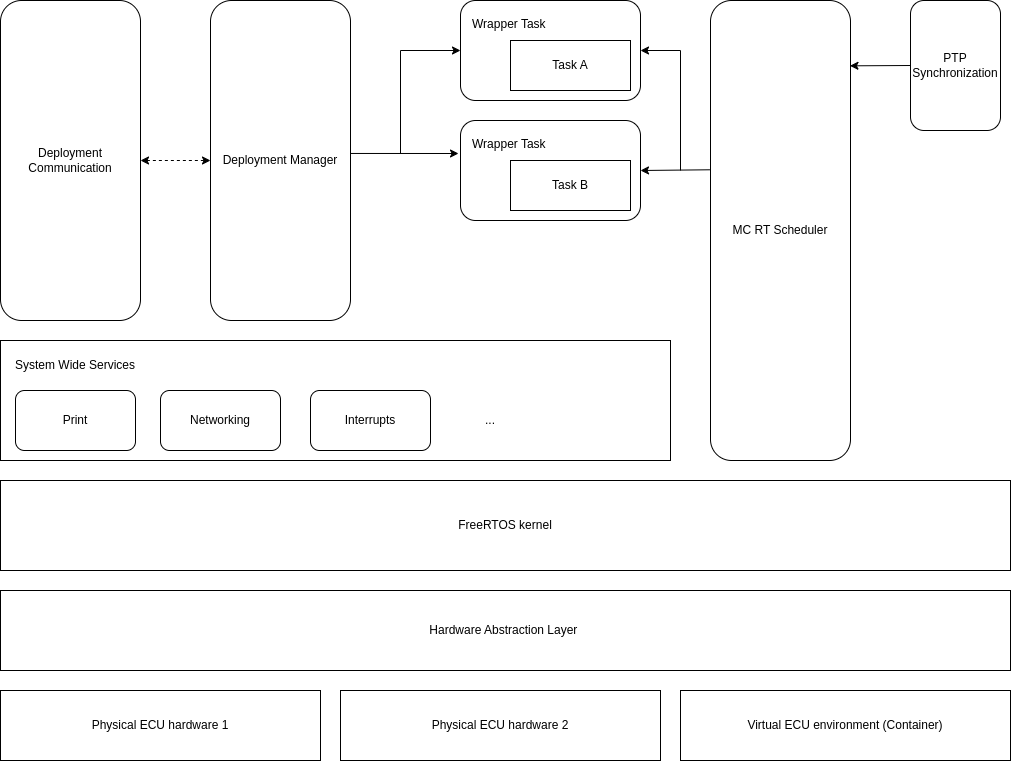
\includegraphics[width=\textwidth]{figures/os_arch_extended.png}}
	\caption{Axcan OS architecture. The FreeRTOS kernel and hardware
	         abstraction layer are used as provided; the remaining components
	         are contributions of this work.}
	\label{fig:os_arch}
\end{figure}

\begin{description}
  \item[Deployment communication.] Maintains the connection to the
    master node, receiving task assignments, executable images and
    checkpoints, and reporting node health and per-task runtime status.
    On a multi-core node only the master core runs this component; the
    remaining sub-nodes run an inter-core variant
    (Section~\ref{subsec:os:multicore}).

  \item[Deployment manager.] Controls the task lifecycle: loading an
    executable into memory, instantiating it, starting and stopping it,
    registering it with the scheduler, monitoring its execution, and
    preparing its state for transfer when a migration event is issued.

  \item[Wrapper task.] The kernel-level thread within which a dynamically
    loaded application executes. It mediates every interaction between the
    application and the rest of the system: it owns the application's memory,
    presents the service interface, invokes the application once per job, and
    performs checkpoint save and restore around that invocation
    (Section~\ref{sec:os:guesttask}).

  \item[Scheduler.] Selects which task executes, according to a configurable
    policy. Axcan OS supports both criticality-agnostic policies
    (rate-monotonic, deadline-monotonic, EDF) and the mixed-criticality
    policies of Section~\ref{sec:os:scheduler}.

  \item[System services.] Provides applications with a minimal API for
    functionality unavailable to a statically linked, dynamically loaded
    binary: console output, networking, memory allocation, and access to
    peripherals. Services are exposed as function pointers resolved at load
    time, which is what permits one binary to run on platforms whose
    underlying implementations differ.
\end{description}

Time synchronisation via PTP, shown in the figure, is a system-wide concern
rather than a component of the node platform; the scheduler's use of it is
described in Section~\ref{subsec:os:timing} and the protocol implementation in
Chapter~\ref{chap:integration}.

Together these components allow any sub-node --- on a physical or a virtual
node, single-core or one core of a multi-core ECU --- to execute a task it was
not compiled with, under real-time constraints, and to participate in
migration.

\subsection{Multi-Core Nodes}\label{subsec:os:amp}

A multi-core ECU runs one instance of Axcan OS per core in an asymmetric
multiprocessing~(AMP) arrangement, as illustrated in
Figure~\ref{fig:multicore_example} for the quad-core ARM Cortex-A53 of the
target hardware. Each instance schedules its own task set independently and is
therefore a sub-node in the sense of Section~\ref{subsec:nodemodel}; tasks are
assigned to sub-nodes, while the ECU as a whole is the node.

\begin{figure}
	\centering
	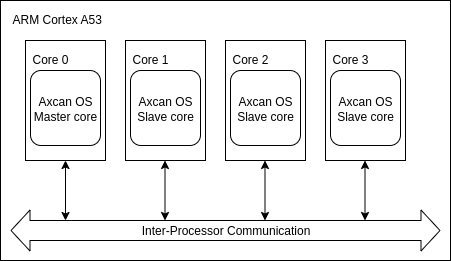
\includegraphics[width=0.5\textwidth]{figures/multicore_example.png}
	\caption{AMP deployment of Axcan OS on the quad-core ARM Cortex-A53 of the
	         target hardware. Each core runs an independent instance and
	         constitutes a node.}
	\label{fig:multicore_example}
\end{figure}

The instances are not quite identical. One core, conventionally core~0, is
designated the \emph{master core}. It is the node's single point of contact
towards the master node, it partitions the task set assigned to the node
across its sub-nodes, and it owns those system services that require exclusive
control of a hardware resource. The remaining \emph{slave cores} reach those
services through an inter-core wrapper interface, and reach the master node
through the master core. Figure~\ref{fig:multicore_deployment_arch} shows the
resulting differences.

\begin{figure}
	\centering
	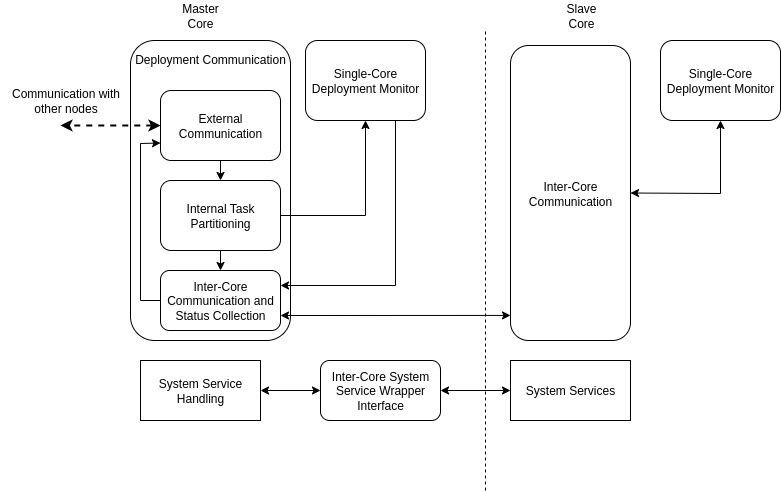
\includegraphics[width=0.75\textwidth]{figures/multicore_deployment_arch.png}
	\caption{Differences between the Axcan OS instances on the master core and
	         on a slave core.}
	\label{fig:multicore_deployment_arch}
\end{figure}

% =====================================================================
\section{Mixed-Criticality Scheduler}\label{sec:os:scheduler}

Requirement~\ref{req:criticality} demands that the guarantees given to a task
of high criticality do not depend on the behaviour of tasks of lower
criticality. On a single node this is a scheduling problem, and it is the
problem this section addresses. Its interaction with migration --- what
happens when a task arrives at a node mid-hyperperiod, and how a mode change
interacts with a migration in progress --- is deferred to
Section~\ref{sec:mig:scheduler}.

\subsection{Baseline: EDF under ESFREE}\label{subsec:os:edf}

The scheduler builds on the policy layer of ESFREE, which replaces the
fixed-priority scheduler of FreeRTOS with one in which priorities are assigned
by a configurable policy. The baseline policy is EDF, which is optimal for
preemptive independent tasks on a uniprocessor in the sense that it schedules
any task set that is schedulable at all~\parencite{liu1973, dertouzos1974}.
Optimality does not survive the introduction of criticality: EDF makes no
distinction between a deadline miss by a high-criticality task and one by a
low-criticality task, and under overload it degrades unpredictably.

\subsection{EDF with Virtual Deadlines}\label{subsec:os:edfvd}

The mixed-criticality policy implemented in Axcan OS is EDF with virtual
deadlines~(EDF-VD)~\parencite{baruah_edfvd}. The system operates in one of the
criticality modes of $\mathcal{L}$, beginning in the lowest. In the low mode,
every task is scheduled; tasks of high criticality are scheduled against a
\emph{virtual} deadline shorter than their true deadline, which reserves
enough slack that they can still meet their true deadlines if the system later
switches to the high mode. If a job of a high-criticality task executes for
longer than its low-mode budget $C_i(\textsf{LO})$, the system switches to the
high mode: low-criticality tasks are suspended or degraded, and
high-criticality tasks revert to their true deadlines with the larger budget
$C_i(\textsf{HI})$.

The virtual deadline of a high-criticality task is obtained by scaling its
true deadline by a factor $x \in (0,1]$ common to all such tasks,
%
\begin{equation}\label{eq:virtualdeadline}
  \hat{D}_i = x \cdot D_i ,
\end{equation}
%
with $x$ chosen so that the task set is schedulable in both modes.
% TODO: state the schedulability condition used, in terms of the low- and
% high-mode utilisations U_LO(LO), U_LO(HI), U_HI(LO), U_HI(HI), and give the
% derivation of the admissible range of x. Baruah et al. give
% x in [U_HI(LO) / (1 - U_LO(LO)), (1 - U_HI(HI)) / U_LO(LO)].
% State explicitly which variant is implemented and any deviation from it.

Note that the deadline used by the scheduler is the virtual deadline of
Equation~\ref{eq:virtualdeadline} applied to the compensated deadline $D_i'$
of Equation~\ref{eq:deadlinecompensation}, not to the global deadline $D_i$.
The two adjustments compose: clock offset and link latency are corrected
first, at the node level and uniformly across its task set, and the virtual
deadline scaling is applied afterwards, at the task level and only to tasks of
high criticality.

\paragraph{Mode changes.} % TODO: expand
The mode-change protocol determines what happens to low-criticality tasks on a
switch to the high mode, and under what condition the system returns to the low
mode. Both choices affect the guarantees the system can offer and must be
stated explicitly.
% TODO: describe (i) the trigger condition for the switch; (ii) the treatment
% of LO tasks -- suspended, or degraded to a longer period; (iii) the
% condition for returning to LO mode (commonly, an idle instant); (iv) whether
% the mode is per-node or system-wide, and if per-node, what this means for a
% distributed system -- this is a question the migration chapter depends on
% and is worth answering here.

\subsection{Realisation Variants}\label{subsec:os:schedvariants}

Two realisations of mixed-criticality scheduling on multi-core ECUs were
developed.

\paragraph{Reserved cores.} Each sub-node is assigned a criticality ceiling
$L_k^{\max}$ (Section~\ref{subsec:criticalitymodel}) and runs plain EDF over
tasks at or below that ceiling. Criticality is thus enforced by partitioning
rather than by the scheduling policy: because no core hosts tasks of differing
criticality, no criticality-induced interference is possible within a core,
and the per-core analysis reduces to ordinary EDF. Sub-nodes reserved for
low-criticality work additionally serve as standby hosts for high-criticality
tasks under the \textsf{HI} migration strategy
(Section~\ref{sec:mig:hi}). The cost is reduced utilisation: capacity on a
high-criticality core cannot be reclaimed by low-criticality work.

\paragraph{Hierarchical virtual-deadline EDF.} A single core hosts tasks of
several criticalities under EDF-VD, with a hierarchical server structure
separating the criticality classes. This permits higher utilisation, at the
cost of a more complex analysis and a mode-change protocol that affects all
tasks on the core.
% TODO: this variant is described in the current draft as a "faulty
% implementation". Decide which of the following the chapter reports:
%   (a) it works, and is evaluated alongside the reserved-core variant;
%   (b) it does not work, and the chapter reports why -- a documented negative
%       result, which is publishable and defensible, but must identify the
%       specific failure (analysis error? mode-change race? server budget
%       replenishment?) rather than leaving it as "faulty";
%   (c) it is out of scope, and the sentence is removed entirely.
% Option (b) is preferable to (c) if the cause is understood.

\subsection{Admission Control}\label{subsec:os:admission}

A node admits a task only if Equation~\ref{eq:admissibility} holds, whose
third conjunct is the local schedulability test. For the reserved-core variant
this is the EDF utilisation bound over the tasks resident on the core; for the
EDF-VD variant it is the two-mode condition of
Section~\ref{subsec:os:edfvd}.
% TODO: state both tests explicitly. Admission control is where the scheduler
% meets migration -- the test run here is the same test the planner must
% model, and Chapter 7 depends on this section stating it precisely.

\subsection{Timing Basis}\label{subsec:os:timing}

The scheduler's notion of time is the node-local clock, synchronised to the
system-wide reference by PTP and bounded in deviation by $\Delta_j$. The
sub-nodes of a node share that clock. Deadlines
arrive from the master node expressed globally and are converted on receipt
according to Equation~\ref{eq:deadlinecompensation}. Because the correction is
uniform across the task sets of all sub-nodes of a node, it preserves the
relative ordering of deadlines and therefore does not alter the sequence of scheduling decisions;
it does, however, consume slack on every task resident on the node. The
implementation of the protocol itself, and the measured behaviour of
$\Delta_j$, are described in Chapter~\ref{chap:integration} and
Chapter~\ref{chap:evaluation} respectively.

% =====================================================================
\section{Dynamic Task Deployment}\label{sec:os:deployment}

A node must be able to execute a task set that is decided at runtime. Two
threads implement this.

The \emph{deployment communication} thread maintains the connection to the
master node. It reports node health and, per task, the number of jobs
completed, the number of deadlines missed, and the time of the last execution.
In the other direction it receives the assigned task set, the executable
images and checkpoints required to start those tasks, and instructions to
start, stop or transfer a task. Received instructions are placed in a shared
memory block from which the deployment manager consumes them.

The \emph{deployment manager} executes those instructions. Starting a task
comprises: receiving the executable image and checkpoint; allocating and
initialising the memory the task requires; loading the image
(Section~\ref{sec:os:loading}); creating the wrapper task that will host it;
and registering the task with the scheduler, which thereafter controls when it
runs. A monitoring sub-thread then checks periodically that the task is
executing correctly and collects the runtime statistics reported by the
communication thread. The monitor is also what stops or pauses a task on
instruction, and what prepares and triggers the transfer of a task's files
when a migration event requires it.

\subsection{Multi-Core Deployment}\label{subsec:os:multicore}

On a multi-core node the master core receives the task set assigned to the
device as a whole and partitions it across the sub-nodes. The partitioning uses a
greedy algorithm that balances load while accounting for the additional
management load carried by the master core itself.
% TODO: state the algorithm precisely, and note that it is deliberately simple
% because the ECU-level assignment has already been made by the planner --
% this is a second-level partitioning, not a scheduling decision.
% TODO: the current draft notes that a criticality-aware extension of this
% partitioning is envisioned. Given the reserved-core variant of
% Section~\ref{subsec:os:schedvariants}, state how the two interact: the
% partitioner must respect the per-core criticality ceilings, which is a
% constraint rather than an extension.

Having partitioned, the master core sends each slave core its share over the
inter-core channel and starts its own share through its deployment manager.
Slave cores replace the deployment communication thread with an inter-core
variant that speaks to the master core rather than to the master node;
everything below that substitution --- the deployment manager, the monitor,
the wrapper tasks, the scheduler --- is identical on every core. Status
reporting is aggregated in the opposite direction: the master core collects
its own status and that of the slave cores and emits a single node-level
report to the master node.

\subsection{Inter-Core Communication}\label{subsec:os:intercore}

Cores communicate through ring buffers in a shared memory region, signalled by
inter-processor interrupts. On this substrate a message-queue abstraction is
provided by the \emph{post office}
library~\parencite{horst, wiesboeck}, which gives each core a
receiving thread that accepts messages into a queue for the corresponding
management thread to process.
% TODO: describe the post office behaviour -- addressing scheme, message
% format, blocking semantics, and what bounds the latency of a transfer.
% This bound matters: it is a component of the migration cost for intra-ECU
% migration (Section~\ref{sec:migrationcost}).

Communication between any pair of cores is possible, although in this
deployment nearly all traffic is between the master core and a slave core.
The exception, and the reason the general case is supported, is the shared
state region used by the \textsf{HI} migration strategy
(Section~\ref{sec:mig:hi}).

% =====================================================================
\section{Cross-Platform Task Loading}\label{sec:os:loading}

Requirement~\ref{req:portability} states that one binary must serve every
admissible node. Axcan OS achieves this with an ELF loader together with a
service abstraction; this section describes both, and
Figure~\ref{fig:multiplatform_tasks} shows the platforms across which a single
binary has been demonstrated to execute.

\begin{figure}
	\centering
	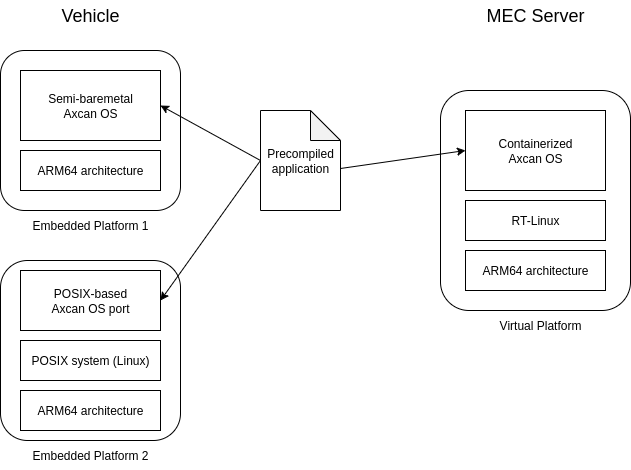
\includegraphics[width=0.6\textwidth]{figures/multiplatform_task_compatibility.png}
	\caption{A single precompiled application executing across a bare-metal
	         embedded platform, a POSIX-hosted platform, and a containerised
	         virtual node, all sharing the ARM~AArch64 architecture.}
	\label{fig:multiplatform_tasks}
\end{figure}

The loader accepts an application compiled as a position-independent
executable, allocates memory for it, performs the necessary relocations, and
transfers control to its entry point. No recompilation is required for
different targets, provided an Axcan OS port runs on the target and the
architecture matches the one the application was compiled for
(\cref{asm:isa}). The loader was implemented in large part in collaboration
with Yinbo Zhou~\parencite{zhou_thesis}.

\subsection{Hardware Abstraction Layer}\label{subsec:os:hal}

Portability of the kernel is not sufficient for portability of applications.
The official FreeRTOS ports abstract the hardware from the kernel, but the
services an application uses --- console output, networking, memory
allocation, peripheral access --- remain reachable only through
platform-specific interfaces. Axcan OS therefore adds an abstraction layer of
its own, with two parts.

The first is the encapsulation of system calls behind uniform signatures.
Each service is exposed to the application through a function pointer with a
platform-independent signature, resolved at load time to whichever
implementation the host platform provides. Because resolution occurs at load
time rather than link time, the application binary carries no dependency on
any particular platform.

The second concerns memory allocation for the loaded image, where the
platforms differ in a way that cannot be hidden behind a signature. On a
bare-metal port, memory may be allocated without regard to the host, though
alignment must respect the target and manual management is required where the
port provides no memory management unit. On a port hosted over POSIX --- the
containerised virtual node, or a development build on a UNIX host --- the
underlying operating system governs memory, and memory obtained through
\texttt{malloc} is not, in general, executable. Allocation there uses
\texttt{mmap} with explicit protection flags, which is more flexible but
requires the loader to manage the mapping explicitly. The loader selects
between the two at build time of the port, not at load time of the
application, so this difference is invisible to the application.

% =====================================================================
\section{The Guest Task Model}\label{sec:os:guesttask}

An application that is to be loaded dynamically, executed under a
mixed-criticality scheduler, and migrated between nodes cannot be an arbitrary
program. This section states the contract it must satisfy and the support
Axcan OS provides. The contract has three parts: how the application is
compiled, how it is structured, and how it declares its state.

\subsection{The Wrapper Task}\label{subsec:os:wrapper}

A loaded application does not execute as a kernel thread of its own. It
executes inside a \emph{wrapper task}: a FreeRTOS thread created by the
deployment manager, one per application, which mediates everything between the
application and the system. The wrapper owns the memory into which the image
was loaded; it holds the service function pointers and the resource table and
passes them to the application at entry; it invokes the application once per
job rather than letting it run freely; and it performs checkpoint restore
before that invocation and checkpoint save after it.

Concentrating these responsibilities in the wrapper is what allows the
application itself to remain an ordinary, statically linked, position-
independent program with no knowledge of the platform, the scheduler, or
migration. It is also what makes a job the unit of scheduling and of
migration: because the wrapper, not the application, controls invocation, the
system has a well-defined point at which the application holds no state
outside its declared structure --- which is precisely the quiescent point
\cref{asm:jobboundary} relies on.

\subsection{Compilation Requirements}\label{subsec:os:compilation}

An application must be compiled as a position-independent executable~(PIE),
and without the standard C library startup code and system call layer that
would bind it to a host. It links instead against a minimal standalone C
library.
% TODO: name the library (newlib, and which configuration) and give the exact
% compiler and linker flags in a listing -- this is the kind of detail a
% reader reproducing the work needs, and it belongs here rather than in an
% appendix.
It must also include the Axcan OS headers, which provide the entry point
handling, the service interface, the resource table, and the checkpoint
mechanism described below.

\subsection{Execution Model and Checkpoints}\label{sec:checkpointing}

Applications are periodic and follow the sense--think--act pattern: the
application's main function constitutes a single job, which reads its inputs,
computes, and produces outputs. Any state that must survive from one job to
the next is loaded at the start of the main function and stored back at its
end. This is the minimal form of the checkpoint mechanism, and under it a
migrated task resumes at a job boundary.

Applications with long-running jobs may declare additional checkpoints within
the body of a job. Each such checkpoint stores the state together with a jump
tag; at the start of the following invocation the tag directs control to the
corresponding point in the code, so that the job resumes from the most recent
completed stage rather than from the beginning. Both forms are shown in
Figure~\ref{fig:user_app_design}.

\begin{figure}
	\centering
	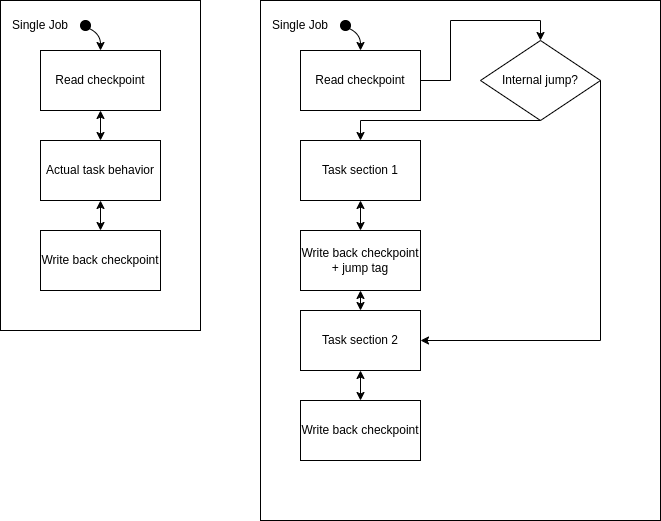
\includegraphics[width=0.6\textwidth]{figures/Task_arch.png}
	\caption{Guest application structure. Left: the minimal form, in which
	         state is restored at the start of a job and stored at its end.
	         Right: the extended form with an intra-job checkpoint and jump
	         tag, permitting resumption from an internal point.}
	\label{fig:user_app_design}
\end{figure}

The state itself is declared by the application as a structure and registered
in a \emph{resource table}, through which the wrapper serialises and restores
it without knowledge of its contents. The correctness of migration therefore
depends on the application declaring its state completely
(\cref{asm:statecapture}); the platform can enforce the mechanism but not the
completeness.

The serialised form of the checkpoint, its metadata and integrity check, and
its use during a migration event are described in
Section~\ref{sec:mig:checkpointtransfer}. This section describes only the
mechanism by which state is captured; its transfer is a matter for
Chapter~\ref{chap:migration}.
% NOTE: this split is deliberate. Chapter 5 owns the guest task ABI, Chapter 6
% owns the wire format and the protocol. Check when revising Chapter 6 that
% the checkpoint description there does not repeat the mechanism described
% here.

% =====================================================================
\section{Memory Management and Isolation}\label{sec:os:isolation}

Section~\ref{sec:safetyscope} states that spatial freedom from interference is
provided only to the extent that the memory protection facilities of the
target hardware are used. This section states what that extent is.

% TODO: this section is a placeholder for content that must be written, and it
% is the section an examiner is most likely to probe. It must answer, plainly:
%
%   (i)   Is the MMU of the Cortex-A53 used to isolate loaded applications
%         from the kernel and from one another? If yes, describe the mapping
%         regime. If no, say so directly.
%   (ii)  What prevents a faulty application from corrupting the memory of
%         another application, of the wrapper, or of the kernel? If the answer
%         is "nothing", that is an acceptable finding for a proof-of-concept
%         platform, but it must be stated, because Requirement R3 is otherwise
%         read as a claim of isolation rather than of scheduling.
%   (iii) What isolates the shared state region used by the HI migration
%         strategy? The design restricts it to tasks of the corresponding
%         criticality -- by what mechanism is that restriction enforced?
%   (iv)  On the POSIX-hosted port, process isolation is provided by the host
%         Linux kernel. Note the asymmetry: the virtual node is in fact
%         better isolated than the physical one.
%
% Framing suggestion: distinguish temporal from spatial freedom from
% interference. The mixed-criticality scheduler provides the former, and that
% is the contribution. The latter is provided partially or not at all, and
% saying so costs nothing while pre-empting the obvious objection.

% =====================================================================
\section{Failure Handling}\label{sec:os:failures}

Dynamic loading introduces failure modes that a statically linked system does
not have. Axcan OS handles them as follows.

% TODO: complete this table from the implementation -- the "---" cells are
% placeholders. Each row should state what the platform does and what it
% reports to the master node, since the master node's recovery action
% (Section~\ref{sec:mig:failure}) depends on distinguishing these cases.
\begin{table}[t]
  \centering
  \caption{Failure modes introduced by dynamic loading and their handling.}
  \label{tab:os:failures}
  \small
  \begin{tabular}{@{}p{0.32\textwidth}p{0.28\textwidth}p{0.28\textwidth}@{}}
    \toprule
    Failure & Detection & Response \\
    \midrule
    Malformed or truncated ELF image      & --- & --- \\
    Unsupported relocation type           & --- & --- \\
    Insufficient memory for the image     & --- & --- \\
    Checkpoint fails its integrity check  & --- & --- \\
    Checkpoint size or version mismatch   & --- & --- \\
    Application faults during a job       & --- & --- \\
    Application overruns $C_i(\textsf{HI})$ & --- & --- \\
    Required service unavailable on node  & --- & --- \\
    \bottomrule
  \end{tabular}
\end{table}

The last two rows connect to the scheduler: an overrun of the high-mode budget
is the trigger for the mode change of Section~\ref{subsec:os:edfvd}, and an
unmet service requirement is a violation of the admissibility condition of
Equation~\ref{eq:admissibility} that should have been prevented by the
master node and is therefore reported as such.

% =====================================================================
\section{Resource Footprint}\label{sec:os:footprint}

Requirement~\ref{req:footprint} constrains the platform to hardware of the
class the architecture targets. Table~\ref{tab:os:footprint} reports the cost
of the additions Axcan OS makes to its base.

% TODO: populate from measurement -- the "---" cells are placeholders. The
% comparison that matters is against stock FreeRTOS on the same port, since
% that isolates the cost of the additions from the cost of the kernel.
\begin{table}[t]
  \centering
  \caption{Static memory footprint of Axcan OS relative to the base kernel,
           ARM Cortex-A53 port.}
  \label{tab:os:footprint}
  \small
  \begin{tabular}{@{}lrr@{}}
    \toprule
    Component & Text (KiB) & Data + BSS (KiB) \\
    \midrule
    FreeRTOS kernel (baseline)      & --- & --- \\
    ESFREE scheduling layer         & --- & --- \\
    Mixed-criticality policies      & --- & --- \\
    Deployment subsystem            & --- & --- \\
    ELF loader                      & --- & --- \\
    Service abstraction             & --- & --- \\
    Inter-core communication        & --- & --- \\
    \midrule
    Total                           & --- & --- \\
    \bottomrule
  \end{tabular}
\end{table}

Per-task cost should be reported alongside: the wrapper task's own stack and
control structures, and the memory reserved for a task's image and state, are
recurring costs that determine how many tasks a node can host and, under the
\textsf{HI} strategy, how many standby copies the system can afford.
% TODO: add a second table or a short paragraph with per-task overhead.

% =====================================================================
\section{Summary}\label{sec:os:summary}

This chapter described Axcan OS, the execution platform on which every node of
the breathable system runs. Built on the FreeRTOS kernel and the ESFREE
scheduling layer, it adds four mechanisms: a mixed-criticality scheduler that
prevents low-criticality tasks from interfering with the timing of
high-criticality ones; a deployment subsystem through which a node receives
and manages a task set decided at runtime; an ELF loader and service
abstraction that allow one binary to execute on bare-metal, POSIX-hosted and
containerised nodes alike; and a guest task model whose wrapper task and
checkpoint mechanism give migration a well-defined quiescent point and a
well-defined unit of state.

Together these satisfy the platform-level obligations of
\cref{req:transfer,req:state,req:criticality,req:portability}: a node can
start a task it was not compiled with, preserve and restore that task's state,
schedule it according to its criticality, and do so identically regardless of
what the node is. What remains --- how a task is moved between two such nodes,
at what cost, and under what conditions the move preserves timing guarantees
--- is the subject of Chapter~\ref{chap:migration}.

The realisation status of the mechanisms described here is stated in
Table~\ref{tab:implstatus}. Axcan OS is a proof-of-concept platform: the set
of system services offered to applications is minimal, the isolation
properties are those of Section~\ref{sec:os:isolation}, and the inter-node
communication mechanisms admit more efficient realisations than the ones
implemented.
